\chapter{Bijlage H}
\label{ch:Bijlage_H_berekeningen}

\section{Relevante constanten}
\label{se:Bijlage_H_relevante_constanten}
\vspace{1 mm}

Wrijvingscoëfficiënt van polyamide-staal (droog) = 	0.3-0.6, \cite{wrijvingscoefficient_rolweerstand_luchtweerstand}\\ 
Hoogte pakket ontvang-afgeef plek = 0.5 m, \cite{beek_2020_opdracht}\\
Afmetingen blokken talud 2 = BxH: 59x156 mm, \cite{beek_2020_opdracht}\\
Maximale versnelling pakkethondje, a = 0.5 $m/(s^2)$\\
Hoek talud 1 = 6,50 graden\\
Hoek van klinker = 3,2 graden\\

\section{Berekening van hoogte massa middelpunt}
\label{se:Bijlage_H_mmp}
\vspace{1 mm}
$ h_{mmp} = h_{0} + (100*m_{a}*h_{p})/(m_{totaal}) $\\
\vspace{1 mm}
    
Waarbij:\\
$h_{mmp} =$ hoogte van het massamiddelpunt, in meters\\
$h_{0} =$ hoogte van het massamiddelpunt zonder het pakketje (wordt uit solidworks gehaald), in meters\\ 
$m_{totaal} =$ massa van het pakkethondje met pakket, 21 kg\\
$m_{a} =$ massa van het pakkethondje, 11 kg\\
$h_{p} =$ hoogte verschil van het massamiddelpunt van het pakket en het pakket hondje\\

    
\begin{figure}[H]
    \centering
    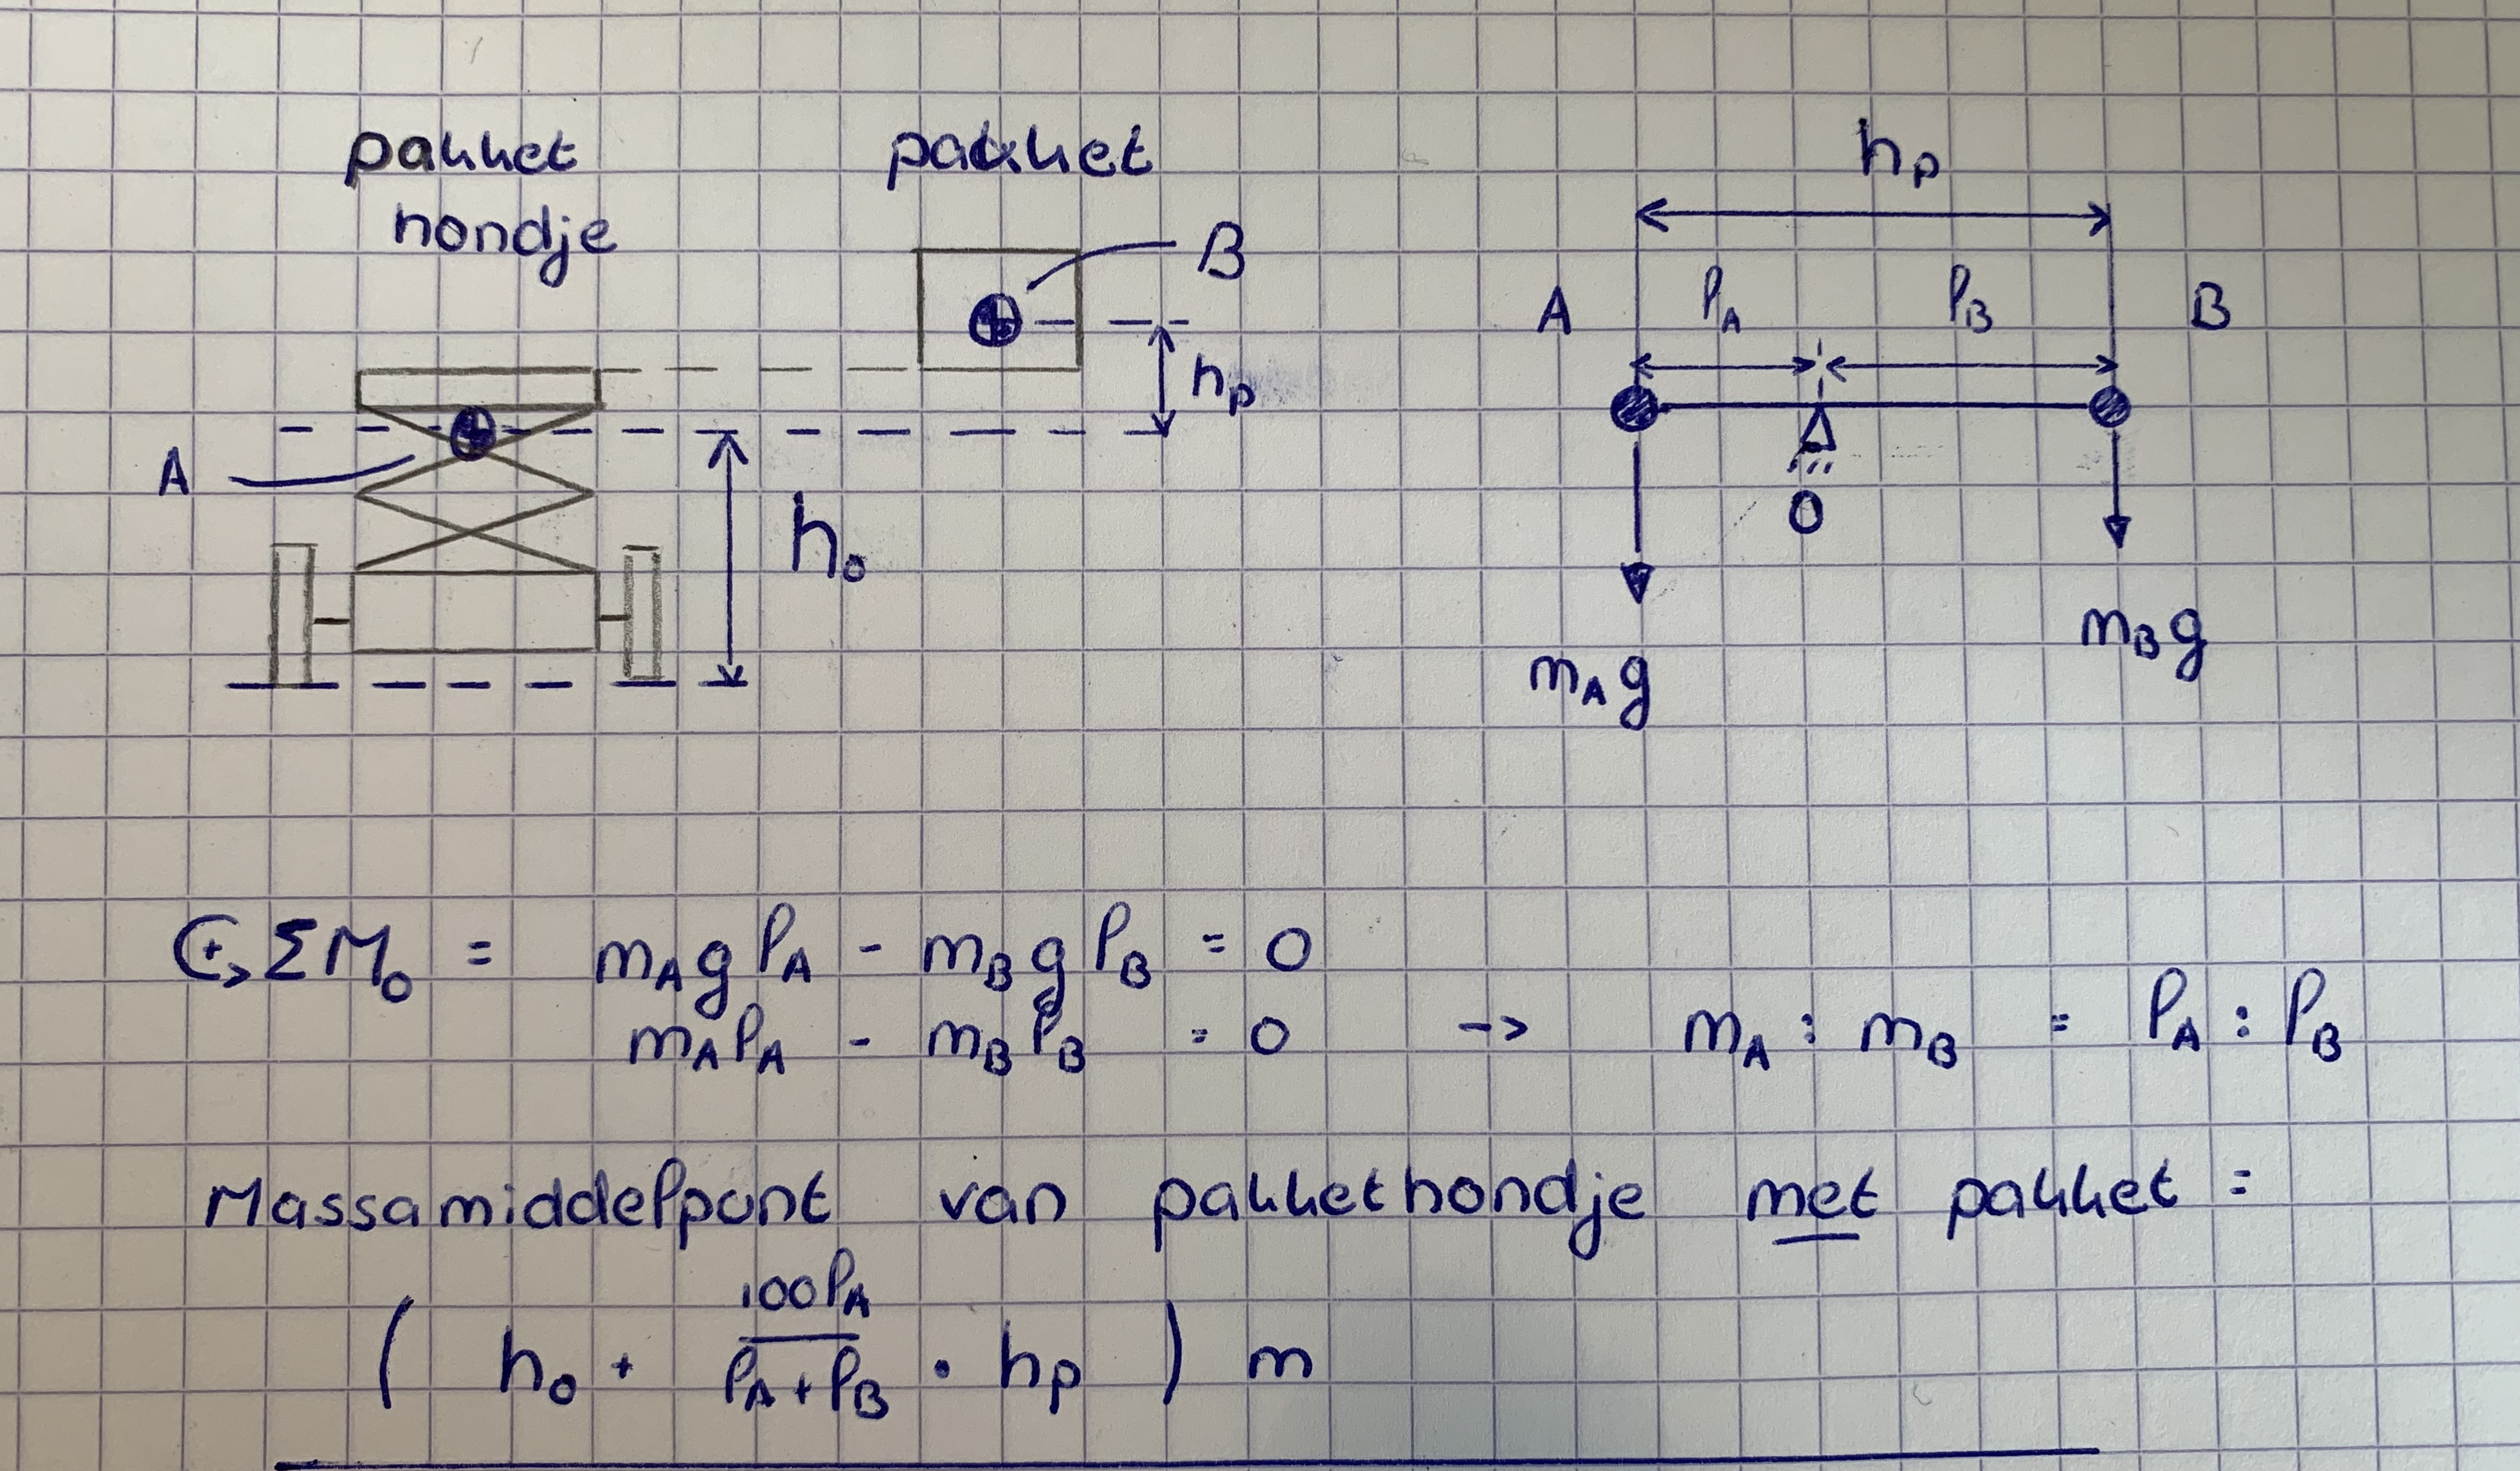
\includegraphics[width = 100mm]{06_Bijlage_H/Dynamische stabiliteit/h_mmp.jpg}
    \caption{bepaling van hoogte van massa middelpunt}
    \label{fig:mmp_h}
\end{figure}

\section{Dynamische stabiliteit}
\label{se:Bijlage_H_Dynamische_stabiliteit}
Tijdens het nemen van de hindernisbaan moet worden gekeken dat het pakkethondje niet omvalt wanneer het zijn maximale versnelling ondervindt, \cref{versnellen_en_remmen}.

\subsection{versnellen en remmen}
\label{versnellen_en_remmen}
In \cref{fig:voorwaarde_talud_nemen} en \cref{fig:voorwaarde_rijden} zijn de voorwaarden te zien die zijn gekoppeld aan de maximale versnelling van het pakkethondje zodat hij niet omvalt.\\
In \cref{fig:voorwaarde_talud_nemen} is te zien dat de verhouding van $a_{max} : g = 1 : 1/3$. Hieruit kan worden opgemaakt dat de maximale versnelling die het pakkethondje mag ondergaan, $a_{max} = 3,27 m/s^2$. Deze waarde is groter dan de daadwerkelijk maximale versnelling van het pakket hondje, zie \cref{se:Bijlage_H_relevante_constanten}, dus het pakket blijft in evenwicht tijdens het nemen van het talud.\\
In \cref{fig:voorwaarde_rijden} is te zien dat de verhouding van $a_{max} : g = 1 : 2.5$. Hieruit kan worden opgemaakt dat de maximale versnelling die het pakkethondje mag ondergaan, $a_{max} = 24,525 m/s^2$. Deze waarde is groter dan de daadwerkelijk maximale versnelling van het pakket hondje, zie \cref{se:Bijlage_H_relevante_constanten}, dus het pakket blijft in evenwicht tijdens het nemen van het talud.\\


\begin{figure}[H]
    \centering
    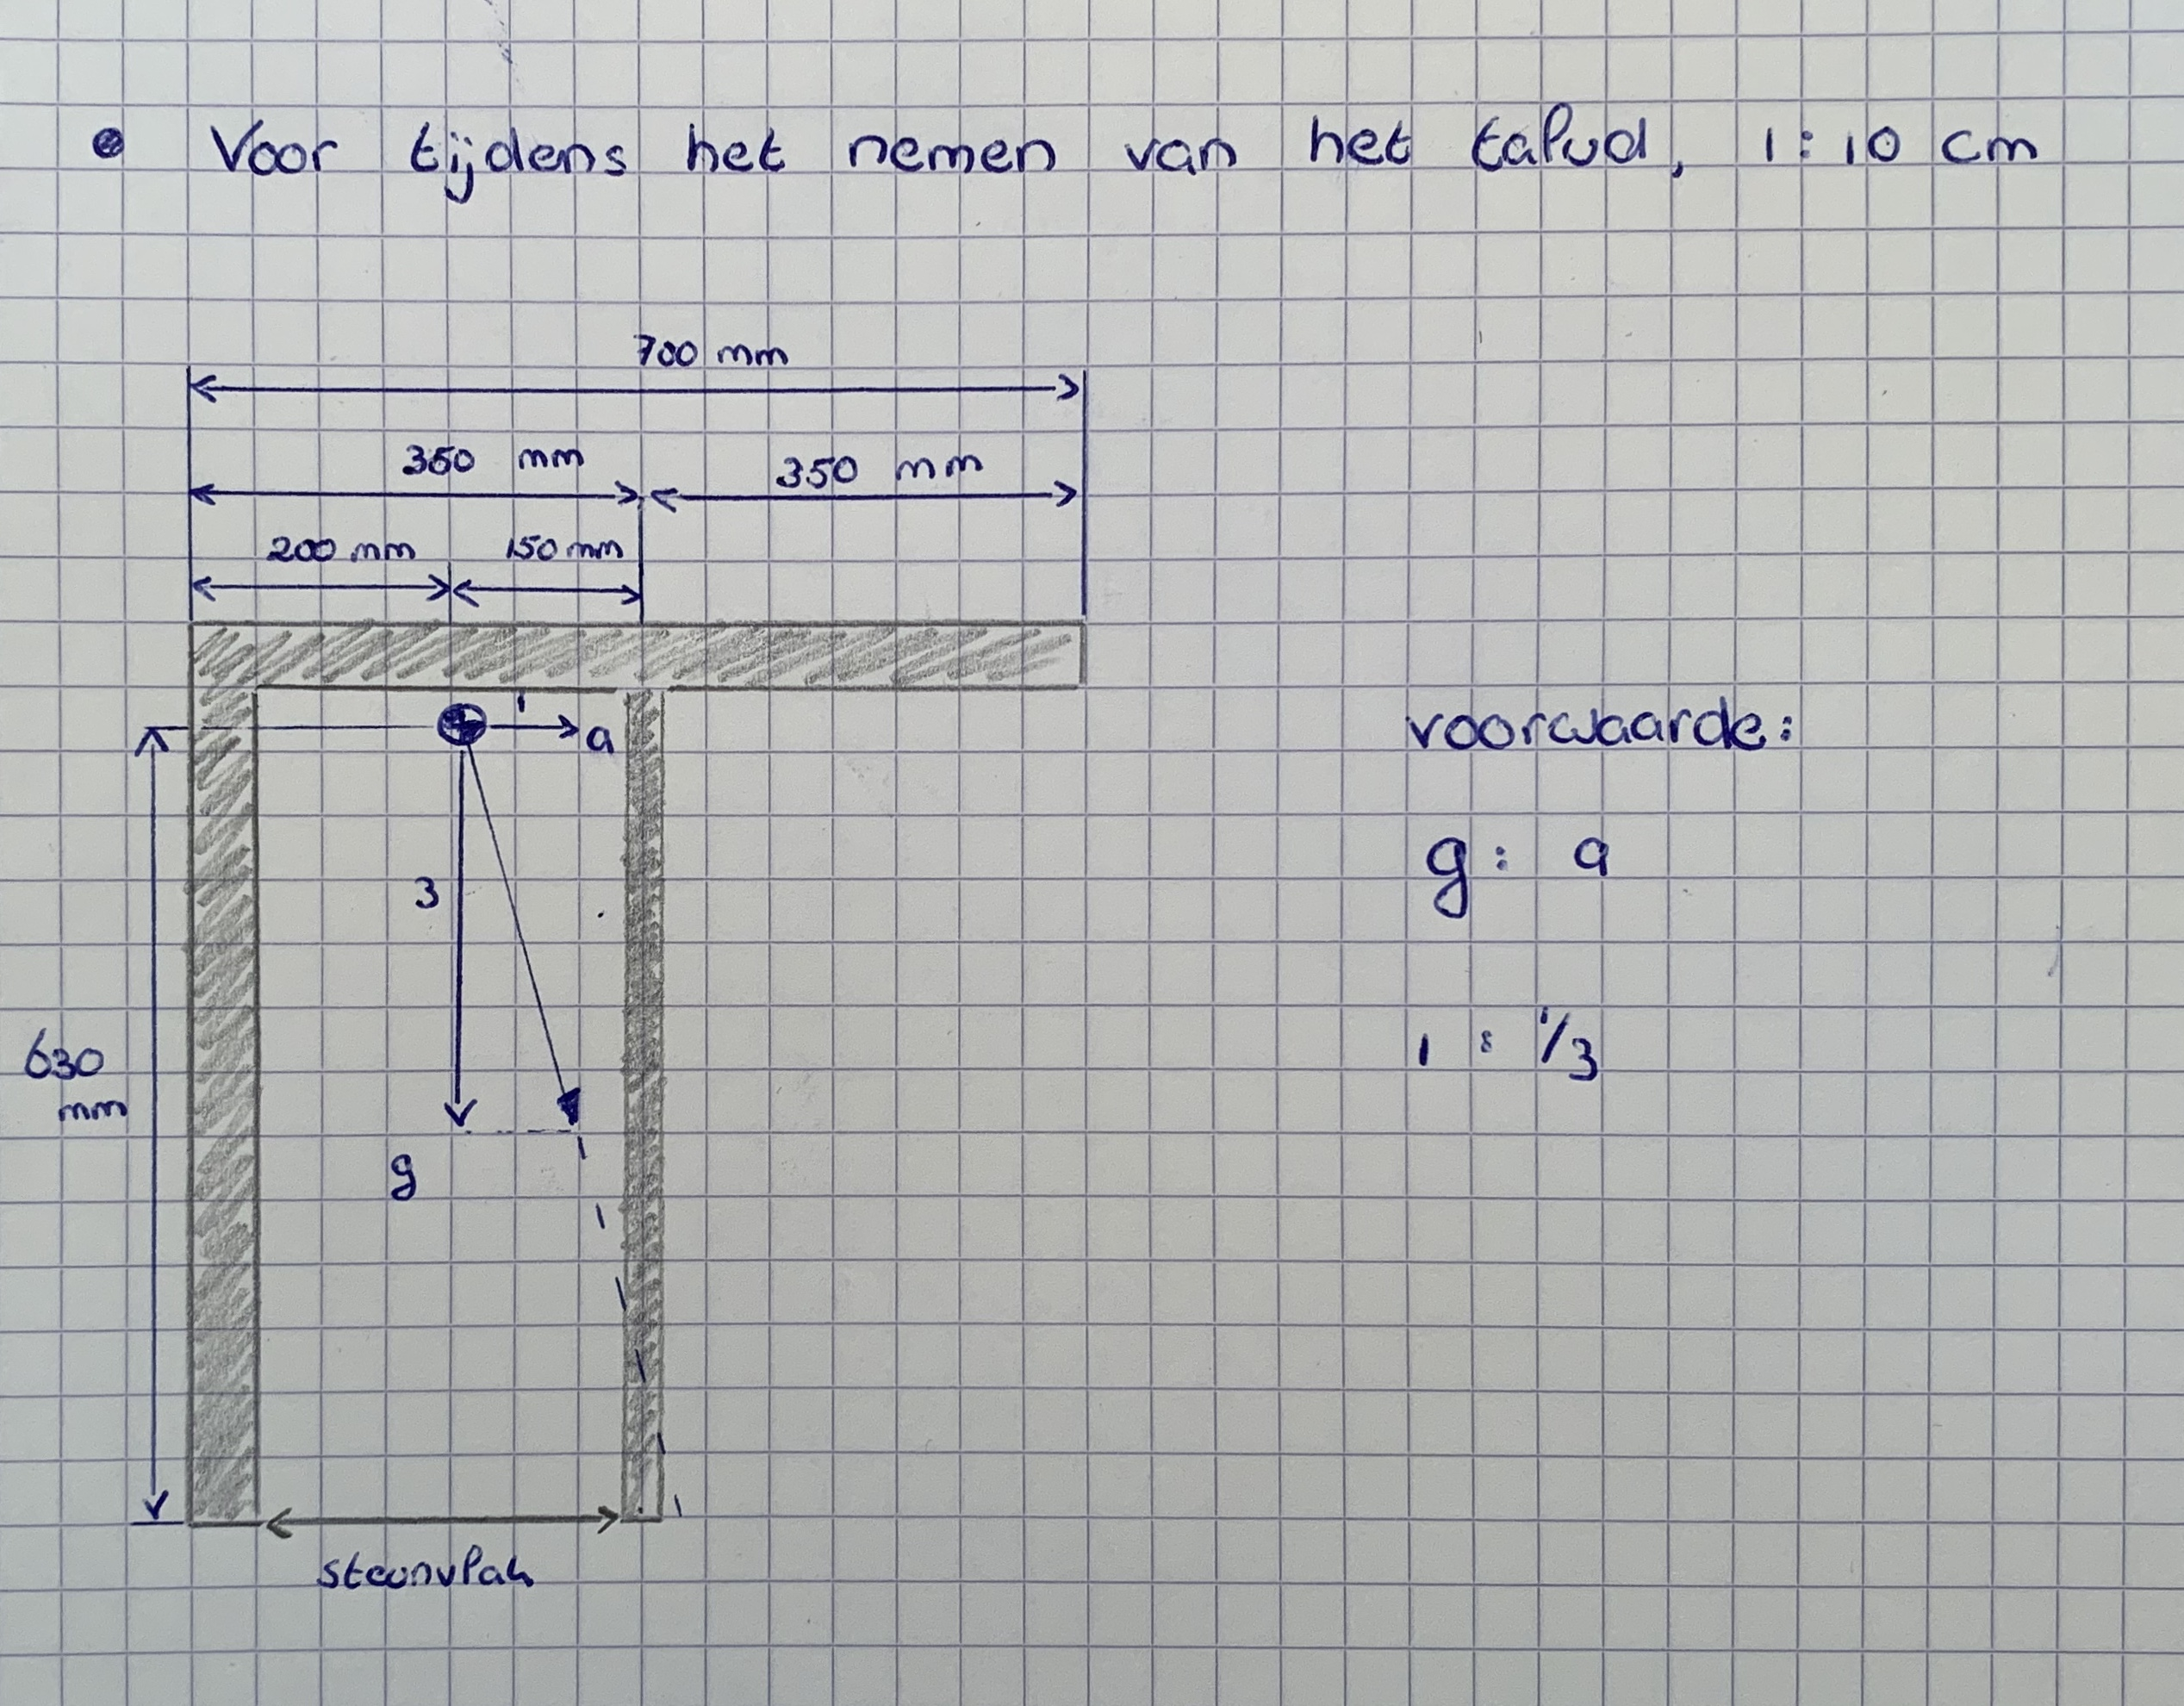
\includegraphics[width = 100mm]{06_Bijlage_H/Dynamische stabiliteit/stabiliteit_talud_nemen.jpg}
    \caption{De stabiliteit voorwaarde van de maximale versnelling tijdens het nemen van het tweede talud}
    \label{fig:voorwaarde_talud_nemen}
\end{figure}

\begin{figure}[H]
    \centering
    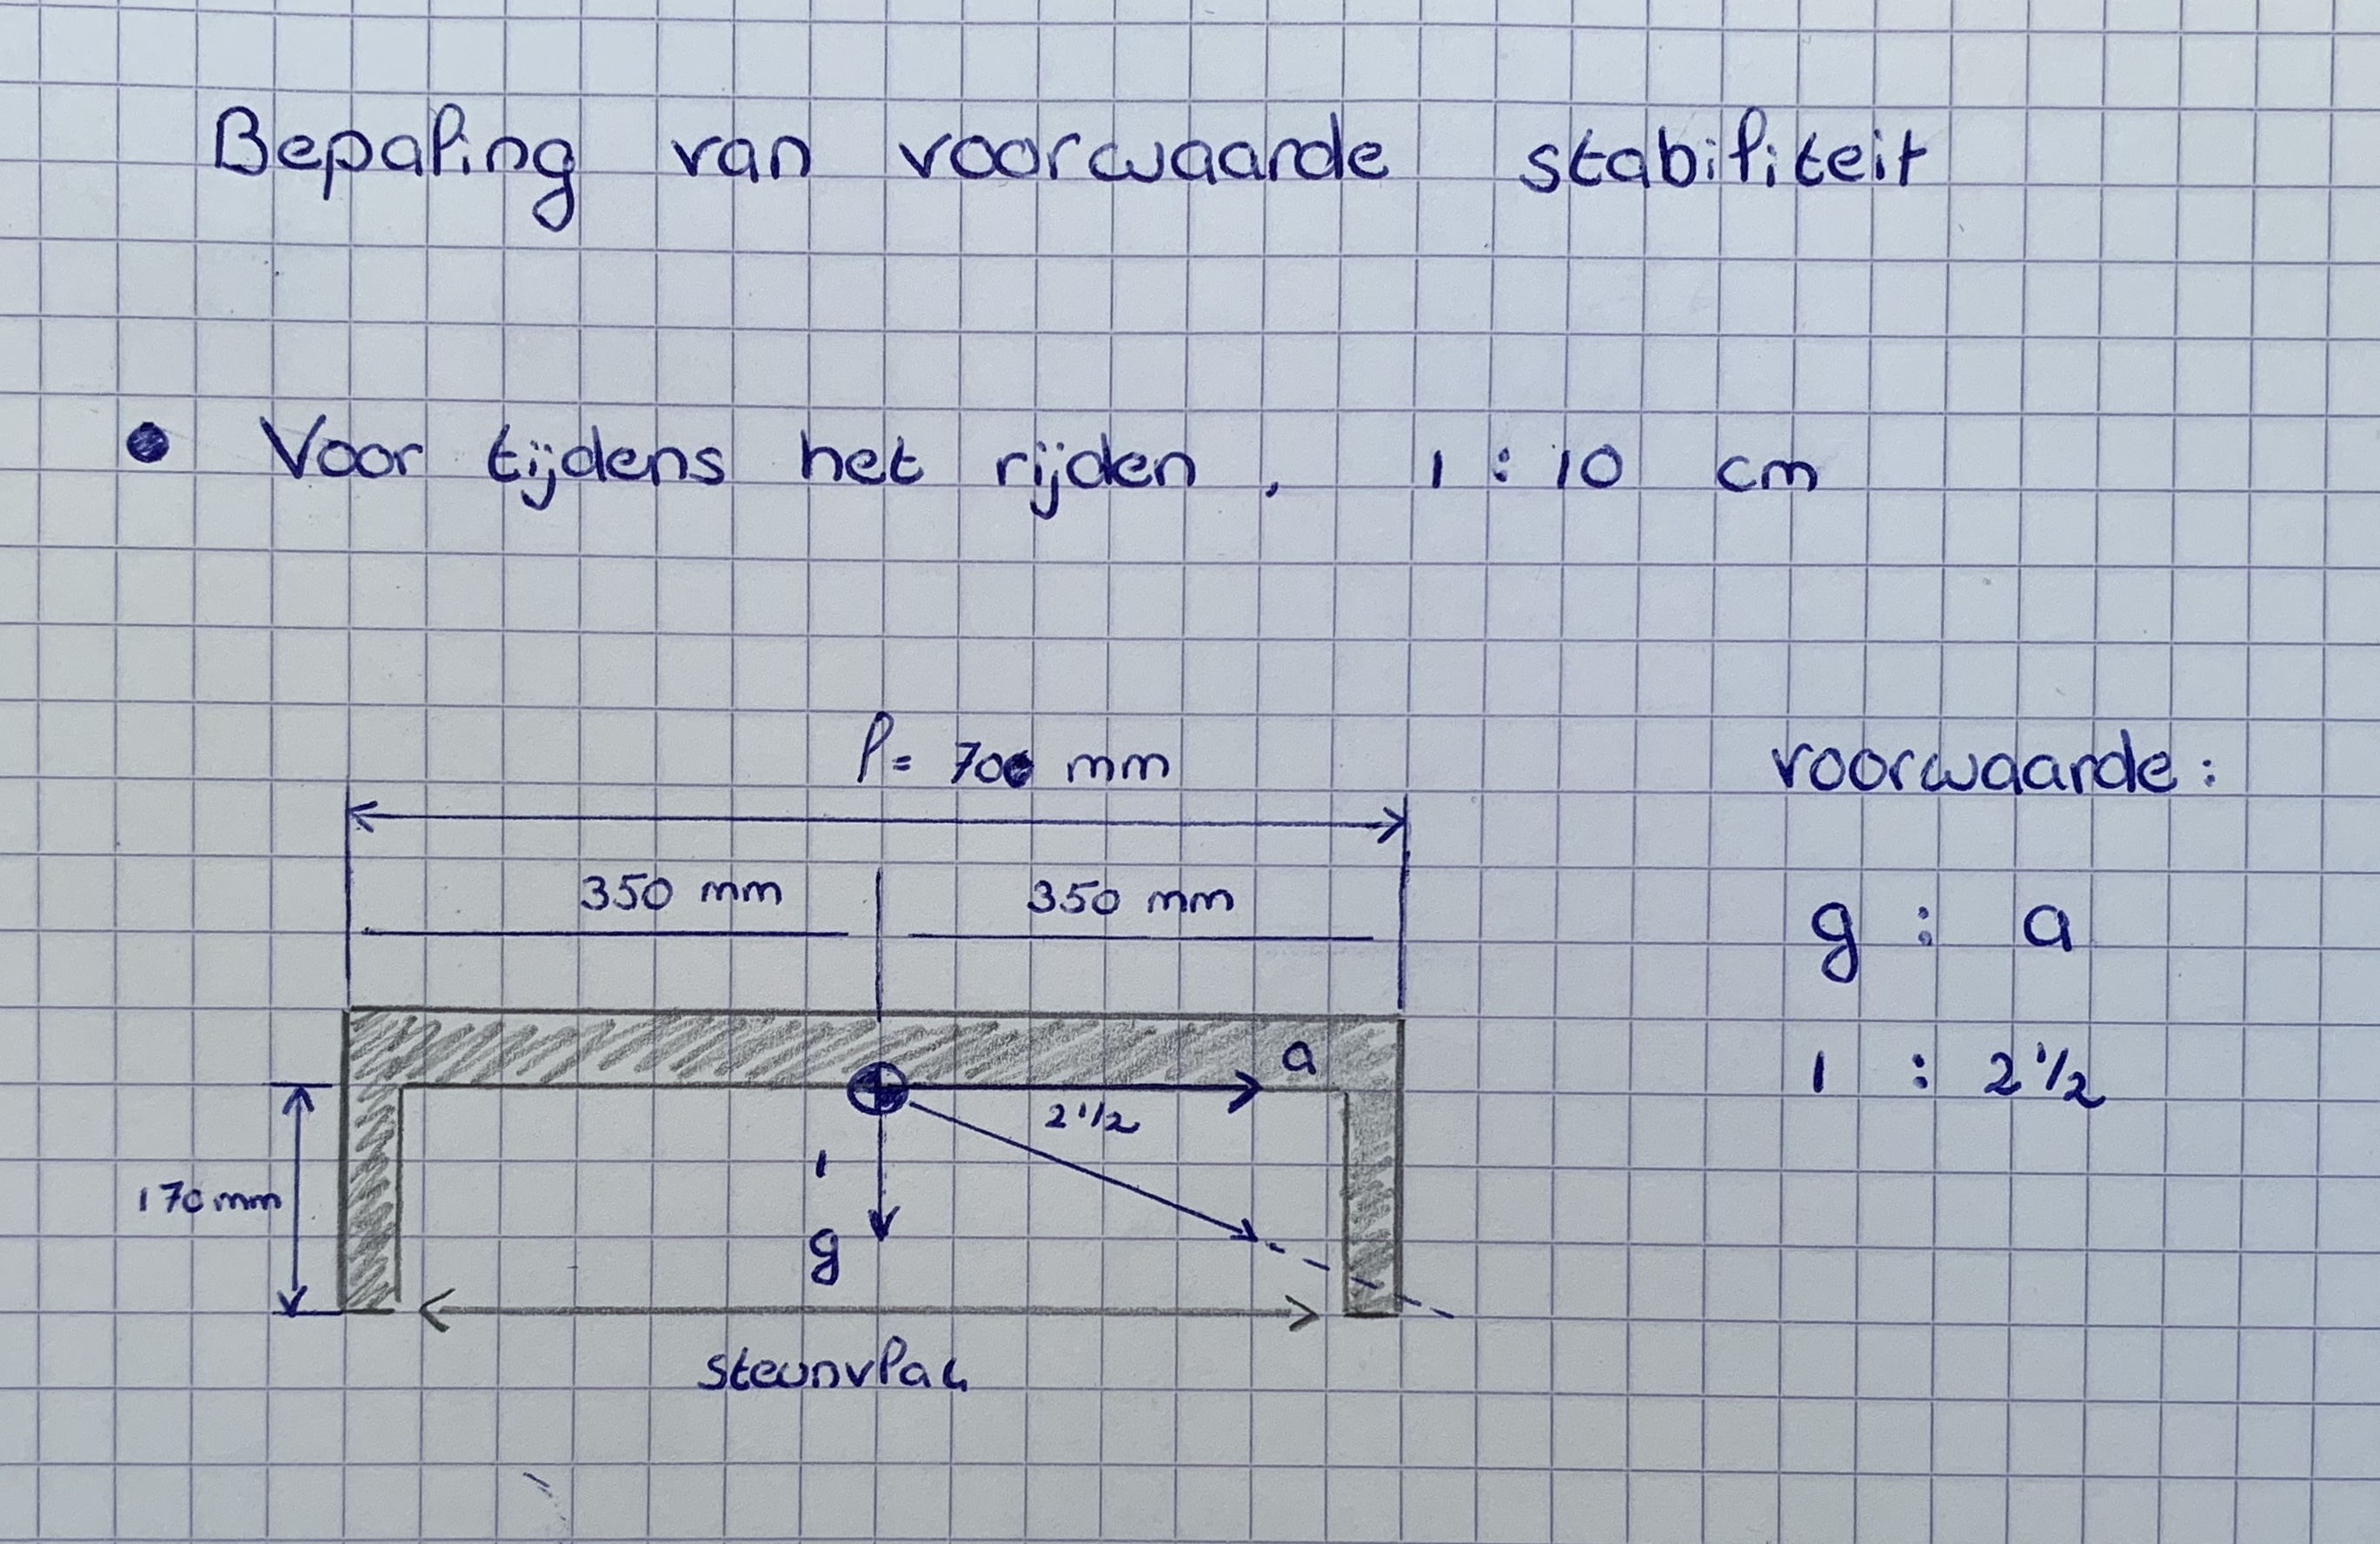
\includegraphics[width = 100mm]{06_Bijlage_H/Dynamische stabiliteit/stabiliteit_rijden.jpg}
    \caption{Dynamische stabiliteit voorwaarde tijdens het rijden van het pakkethondje}
    \label{fig:voorwaarde_rijden}
\end{figure}


\section{Statische stabiliteit}
\label{se:Bijlage_H_Statische_stabiliteit}
Het pakkethondje mag niet omvallen tijdens het nemen van het eerste talud of omvallen door hoek die de klinkers maken met het pakket hondje. In \cref{se:sub_talud1_statisch} staat de berekening voor de statische balans tijdens het nemen van het eerste talud. In \cref{se:sub_rijden_statisch} staat de berekening van de statische balans tijdens het rijden.

\subsection{Nemen van talud 1}
\label{se:sub_talud1_statisch}

Het pakket hondje is ontworpen met een lengte van 350 mm tussen elke poot en een verrolbaar massamiddelpunt. Dit zorgt ervoor dat het massa middelpunt ten alle tijden boven het steunvlak blijft tijdens het nemen van het talud. Hierdoor blijft het pakket altijd in evenwicht.\\

\subsection{Tijdens het rijden}
\label{se:sub_rijden_statisch}
In \cref{fig:balans_hoek} is te zien dat de waarde voor $x_{mmp}$ niet kleiner mag worden dan 0. Omdat het figuur op school is af te lezen kan worden bepaald dat de hoek $\alpha$ groter moet worden dan 45 graden, dit is in deze situatie niet het geval dus het pakket hondje blijft in balans.\\

\begin{figure}[H]
    \centering
    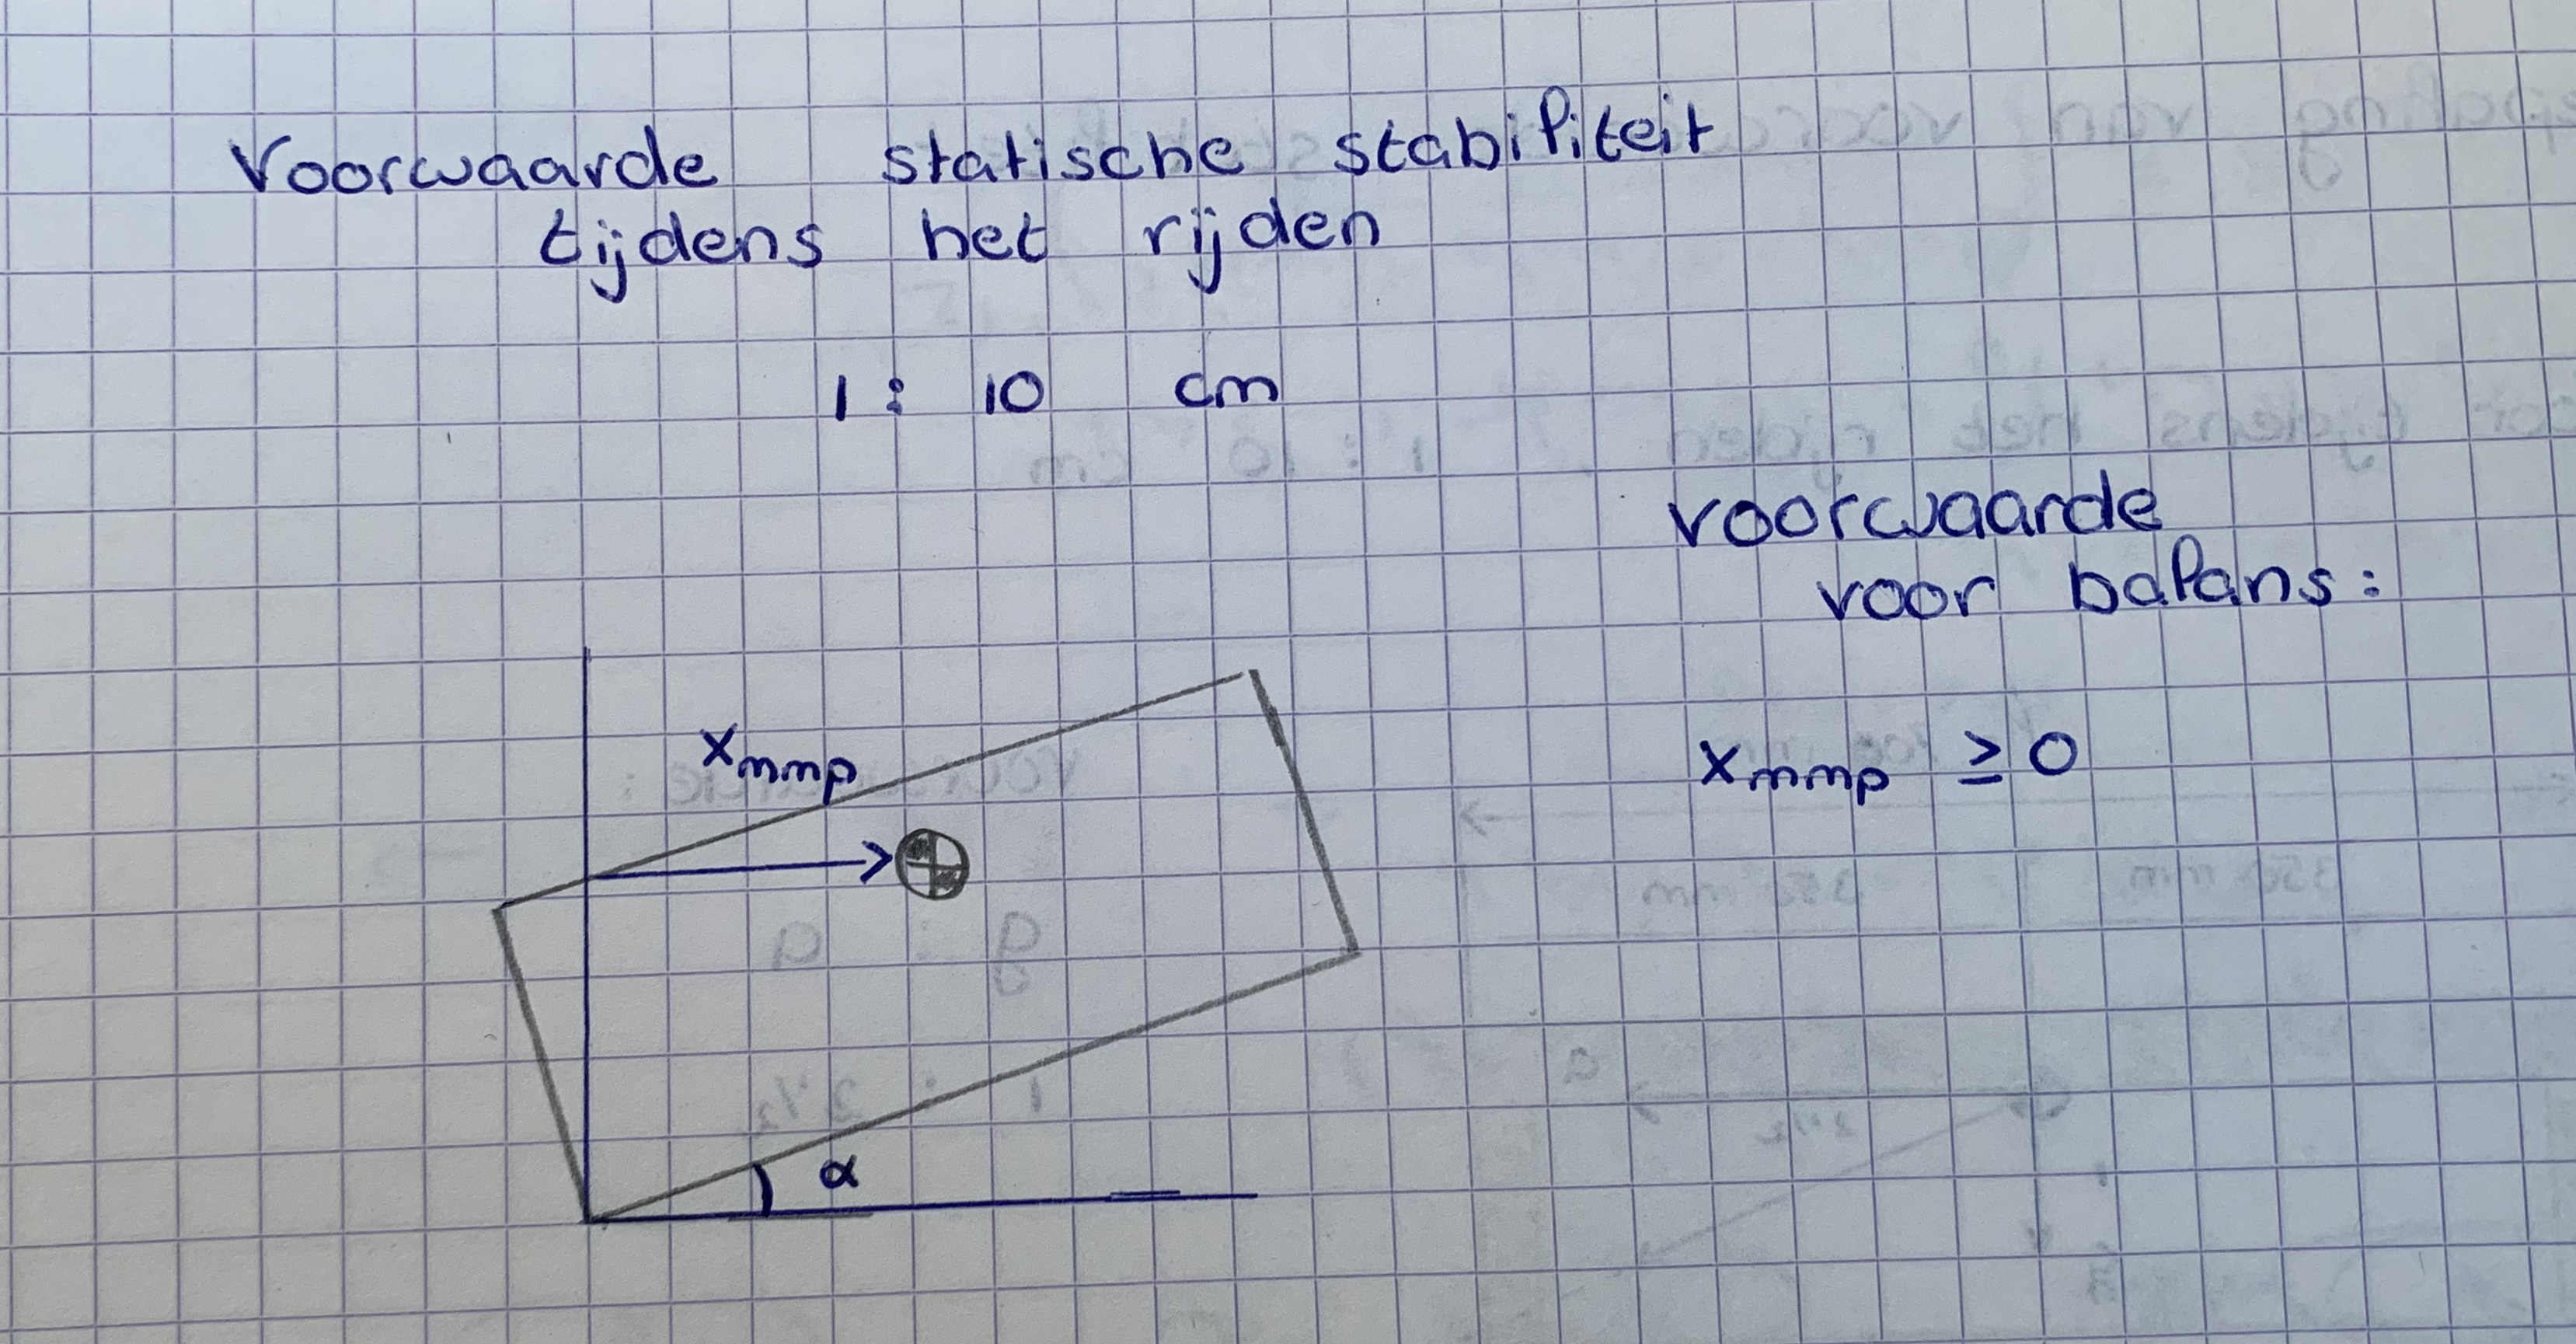
\includegraphics[width = 100mm]{06_Bijlage_H/Dynamische stabiliteit/balans_hoek.jpg}
    \caption{Statische stabiliteit voorwaarde tijdens het rijden van het pakkethondje}
    \label{fig:balans_hoek}
\end{figure}


\section{Balans van het pakketje}
\label{se:Bijlage_H_balanspakket}
Tijdens het vervoeren van het pakket is het ook essentieel om te bepalen of het pakket niet van het platform afglijdt tijdens het nemen van het eerste talud, \cref{se:sub_balans_talud1}, en om te kijken naar de balans van het pakket tijdens het rijden over de klinkers, \cref{se:sub_balans_rijden}.

\subsection{Nemen van Talud 1}
\label{se:sub_balans_talud1}

In \cref{fig:balans_pakket} kan worden gezien dat de voorwaarde voor evenwicht is:\\
$\mu_{s} \leq tan(\alpha) $\\ 
\vspace{\baselineskip}
Hieruit volgt dat $tan(6,5) \leq 0.3$, dus het pakket blijft in evenwicht is.

\subsection{Rijden}
\label{se:sub_balans_rijden}

In \cref{fig:balans_pakket} kan worden gezien dat de voorwaarde voor evenwicht is:\\
$\mu_{s} \leq tan(\alpha) $\\ 
\vspace{\baselineskip}
Hieruit volgt dat $tan(3,2) \leq 0.3$, dus het pakket blijft in evenwicht is.

\begin{figure}[H]
    \centering
    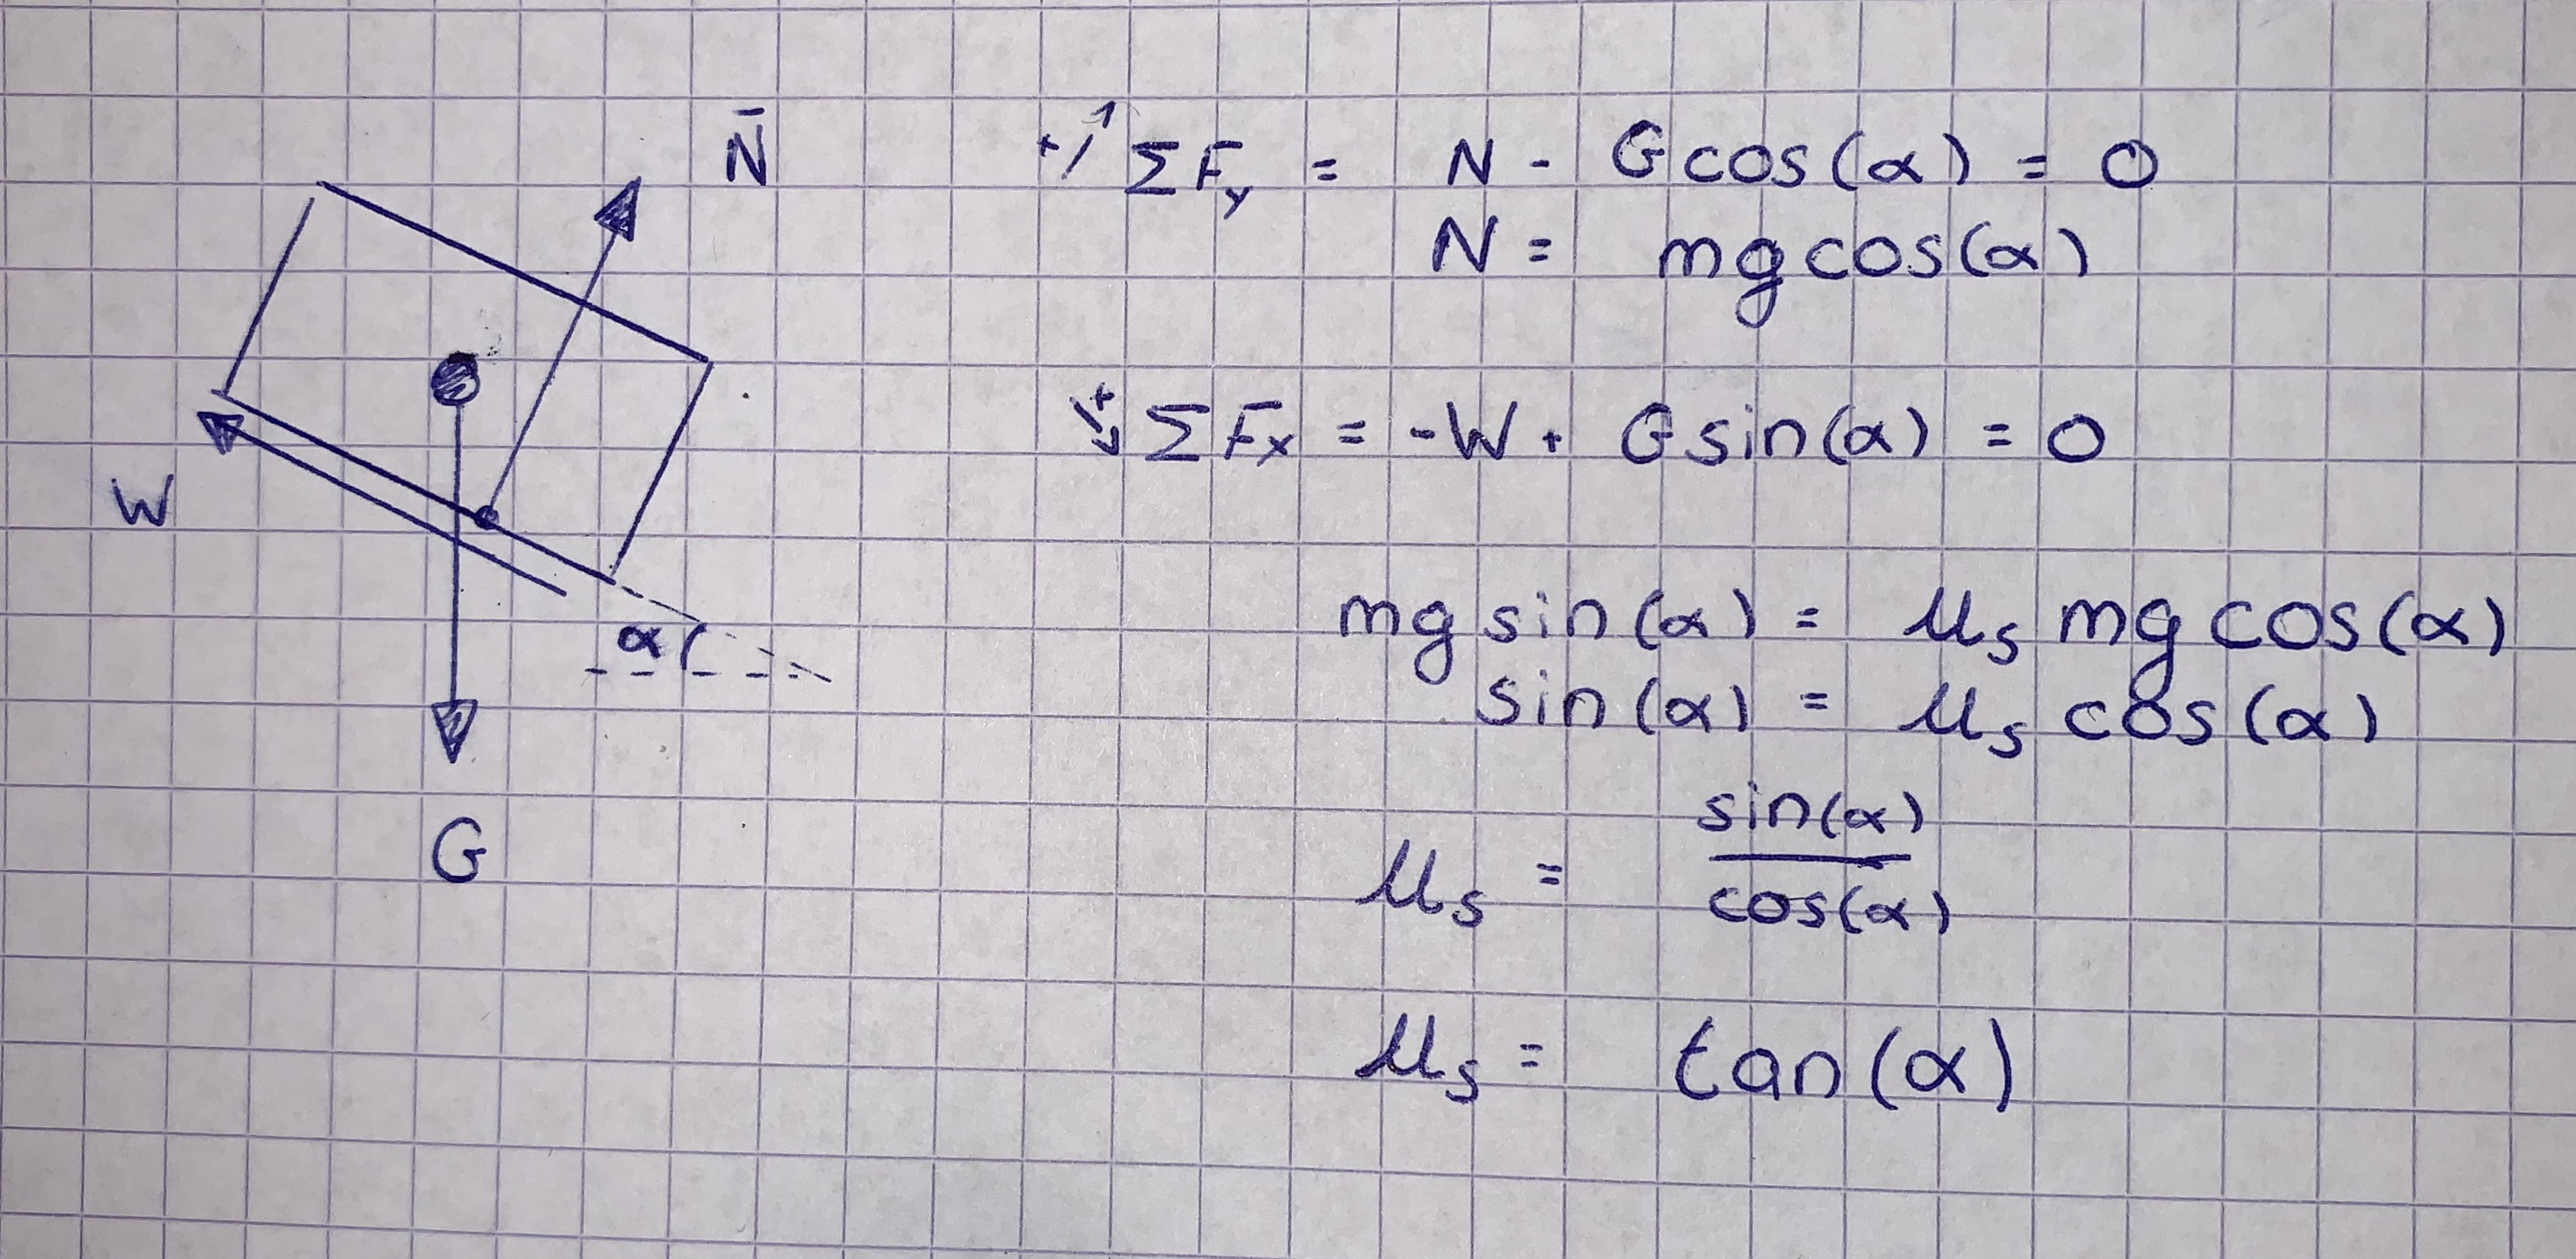
\includegraphics[width = 100mm]{06_Bijlage_H/balans_pakket.jpg}
    \caption{balans van pakket}
    \label{fig:balans_pakket}
\end{figure}

\section{Berekeningen batterijcapaciteit}

Men begint met de volgende elementaire formules: (\cite{giancoli_2014})

\begin{equation}
    P = U \cdot I
    \label{eq:spanning}
\end{equation}
\begin{equation}
    E = P \cdot \Delta t
    \label{eq:energie}
\end{equation}

Waarbij:\\
$E$ de energie is in Joule, \\
$U$ de spanning in Volt,         \\
$I$ de stroom in Ampère,         \\
$P$ het vermogen in Watt,        \\
$\Delta t$ de tijd in seconden. 

\vspace{\baselineskip}

Uit de motorkarakteristiek (\cite{motraxx-elektrogeraete-gmbh}) kan men bepalen wat de nominale spanning is en de bijbehorende stroom van de DC motoren voor de aandrijving. De spanning is $12 V$ en de stroom is $0.35 A$. Het vermogen is dan volgens \cref{eq:spanning} $4.2 W$.

Het is lastiger om voor de stepper motoren een exacte energie-berekening te maken omdat zij ook als ze niet draaien energie gebruiken. Wel weten we de ingangspanning van 18V en een maximale stroom van 2A door de stepper drivers. Samen zorgt dit volgens \cref{eq:spanning} voor een piekvermogen van 36W per stepper motor. 

Voor de verdere elektronica is er nauwelijks stroom nodig. De arduino zou op een 9V batterij kunnen werken dus deze wordt niet mee genomen in de berekening.

In totaal is het piekvermogen van het pakkethondje met drie stepper en twee DC motoren dus 116W. Om dit de maximale tien minuten aan te drijven is volgens \cref{eq:energie} een accu met een capaciteit van $70KJ$ nodig. 

De capaciteit van de accu is gelijk aan 3 Ah bij 18V, wat gelijk staat aan $54Wh$ en $195KJ$. De accu heeft dus ruim voldoende capaciteit om de motoren te laten draaien.


\section{DC Motorkaraktiristiek}

\begin{figure}[H]
    \centering
    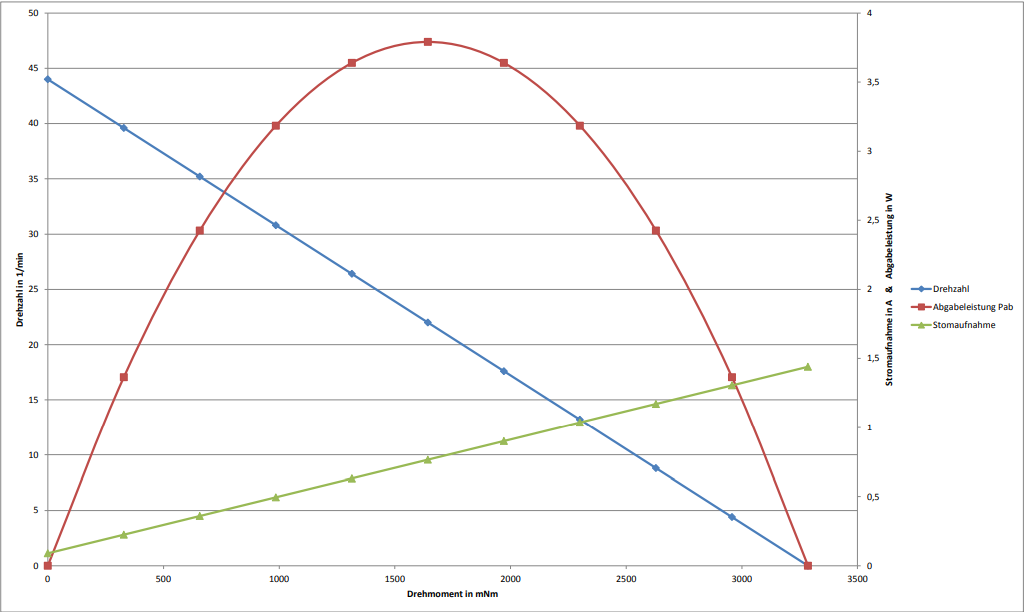
\includegraphics[width=150mm]{06_Bijlage_H/motorkariskiristiek.png}
    \caption{Motorkaraktiristiek van de gekozen DC motor voor de aandrijving. (cite{motraxx-elektrogeraete-gmbh})}
    \label{fig:motorkaraktiristiek}
\end{figure}

